% Provenance (never printed): cycle 3 "Matiere, mouvement, energie,
% information" and "La planete Terre" (meteorological phenomena, the water in
% the air, measuring the weather); see sources/book1/PROVENANCE.md.
% Book 1, grade 4, chapter 1.
\chapter{Nubes, lluvia y nieve}\label{ch:g4:clouds-rain-snow}

Es una tarde calurosa de verano. A mediodía el cielo estaba azul, con unas
pocas nubecillas blancas como bolas de algodón. A las tres, una de ellas ha
crecido. Se hincha hacia arriba, cada vez más alta, como una coliflor
blanca sobre una base gris y plana. Su cima se extiende. Su base se
oscurece. Sopla una ráfaga de viento fresco, caen las primeras gotas
gordas, y durante veinte minutos llueve a cántaros. Después la \omterm{def:g4:clouds-rain-snow:cloud}{nube} se
aleja, vuelve el sol y las aceras mojadas echan vapor.

¿De dónde salió esa \omterm{def:g4:clouds-rain-snow:cloud}{nube}? ¿De qué está hecha? ¿Y cuánta \omterm{def:g4:clouds-rain-snow:precipitation}{lluvia} cayó en esos
veinte minutos?

\begin{recall}
El \omterm{def:g1:watching-the-weather:weather}{tiempo} es el estado del aire en un lugar y un momento dados: soleado,
nublado, lluvioso, con \omterm{def:g4:clouds-rain-snow:precipitation}{nieve}, con viento, con \omterm{def:g4:clouds-rain-snow:cloud}{niebla}; lo anotamos en una
\omterm{def:g1:watching-the-weather:weather-chart}{tabla del tiempo} (\cref{ch:g1:watching-the-weather}). El agua del \omterm{def:g2:water-on-earth:ocean}{mar}, de
los \omterm{def:g1:landscapes-around-us:water}{lagos} y del suelo sube al aire y vuelve a bajar en forma de \omterm{def:g4:clouds-rain-snow:precipitation}{lluvia}
(\cref{ch:g2:water-on-earth}). Los libros de física cuentan cómo el agua se
evapora (de líquido a un gas invisible), se condensa (de gas a gotitas de
líquido otra vez) y se congela (de líquido a hielo), y cómo un termómetro
mide la temperatura en grados Celsius.
\end{recall}

\section{¿Qué es una nube?}

El aire que nos rodea siempre contiene algo de agua, en forma de un gas
invisible: el vapor de agua. Cuando el aire sube, se enfría. Cuando se
enfría lo suficiente, parte de su vapor de agua se condensa en gotitas de
agua tan diminutas que el más leve soplo de aire las mantiene flotando.
Miles de millones de esas gotitas, unas junto a otras, forman una \omterm{def:g4:clouds-rain-snow:cloud}{nube} que
podemos ver. Muy arriba, donde el aire está muy frío, las gotitas se
congelan y la \omterm{def:g4:clouds-rain-snow:cloud}{nube} está hecha de trocitos diminutos de hielo.

\begin{definition}[Nube y niebla]\label{def:g4:clouds-rain-snow:cloud}
Una \emph{nube}\index{nube} es un gran número de gotitas diminutas de agua,
o de trocitos diminutos de hielo, que flotan juntos en el aire. La
\emph{niebla}\index{niebla} es una nube que toca el suelo.
\end{definition}

\begin{example}[Tu aliento una mañana fría]\label{ex:g4:clouds-rain-snow:breath}
Una mañana fría, tu aliento forma una nubecilla blanca delante de la boca.
El aire que echas es cálido y contiene vapor de agua. El aire frío lo
enfría enseguida, el vapor se condensa en gotitas diminutas --- y aparece
una \omterm{def:g4:clouds-rain-snow:cloud}{nube} en miniatura, que luego se desvanece cuando las gotitas vuelven a
evaporarse.
\end{example}

Una \omterm{def:g4:clouds-rain-snow:cloud}{nube} es blanca porque sus gotitas desvían la luz del Sol en todas las
direcciones. Cuando es muy espesa, llega poca luz hasta su base, y vista
desde abajo parece gris, o casi negra: es la señal de una \omterm{def:g4:clouds-rain-snow:cloud}{nube} cargada,
llena de agua.

\section{Las familias de nubes}

Las \omterm{def:g4:clouds-rain-snow:cloud}{nubes} tienen muchas formas, y los observadores del \omterm{def:g1:watching-the-weather:weather}{tiempo} de todo el
mundo las clasifican de la misma manera: por su forma y por la altura a la
que flotan.

\begin{definition}[Familias de nubes]\label{def:g4:clouds-rain-snow:cloud-families}
Las cuatro familias de \omterm{def:g4:clouds-rain-snow:cloud}{nubes} que hay que conocer son:
\begin{itemize}
  \item los \emph{cúmulos}\index{cumulo@cúmulo}: \omterm{def:g4:clouds-rain-snow:cloud}{nubes} amontonadas,
        blancas y esponjosas, de base plana, como bolas de algodón;
  \item los \emph{estratos}\index{estrato}: \omterm{def:g4:clouds-rain-snow:cloud}{nubes} en capa, una lámina gris
        y plana que cubre todo el cielo, a poca altura;
  \item los \emph{cirros}\index{cirro}: \omterm{def:g4:clouds-rain-snow:cloud}{nubes} deshilachadas, finos hilos o
        rizos blancos, muy altos, hechos de hielo;
  \item los \emph{cumulonimbos}\index{cumulonimbo}: la \omterm{def:g4:clouds-rain-snow:cloud}{nube} de tormenta,
        una torre enorme que se eleva desde una base baja y oscura hasta
        una altura muy grande, y cuya cima suele extenderse en plano.
\end{itemize}
\end{definition}

Los nombres vienen del latín: \emph{cumulus} significa montón,
\emph{stratus} capa, \emph{cirrus} rizo de pelo y \emph{nimbus} \omterm{def:g4:clouds-rain-snow:cloud}{nube} de
\omterm{def:g4:clouds-rain-snow:precipitation}{lluvia}.

\begin{omfigure}
\begin{minipage}[b]{0.49\linewidth}\centering
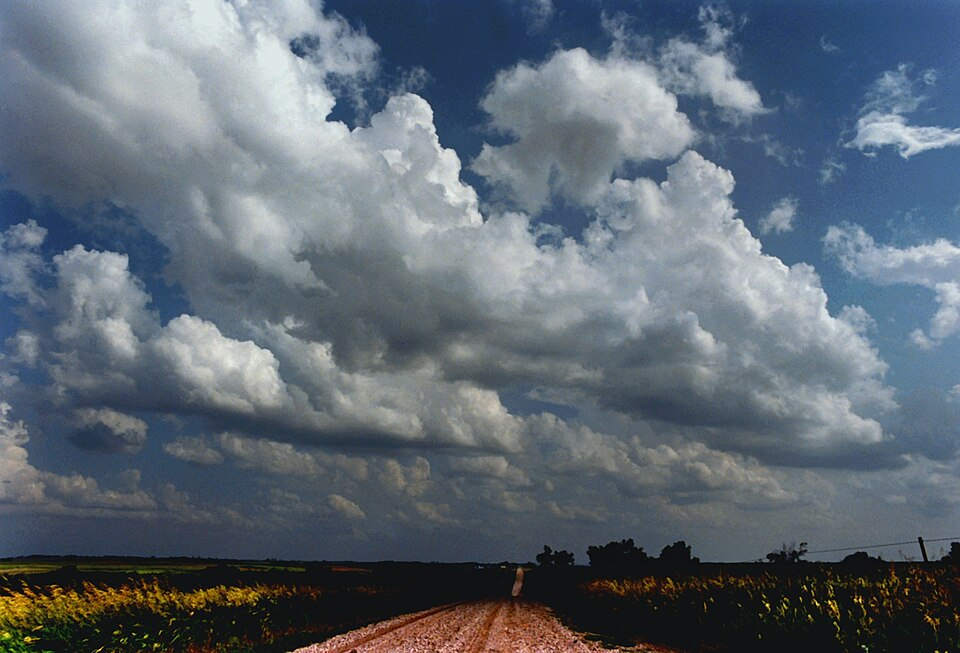
\includegraphics[width=\linewidth]{images/book1/g4-cumulus.jpg}

{\small \omterm{def:g4:clouds-rain-snow:cloud-families}{Cúmulos}, \omterm{def:g4:clouds-rain-snow:cloud}{nubes} amontonadas de base plana.}
\end{minipage}\hfill
\begin{minipage}[b]{0.49\linewidth}\centering
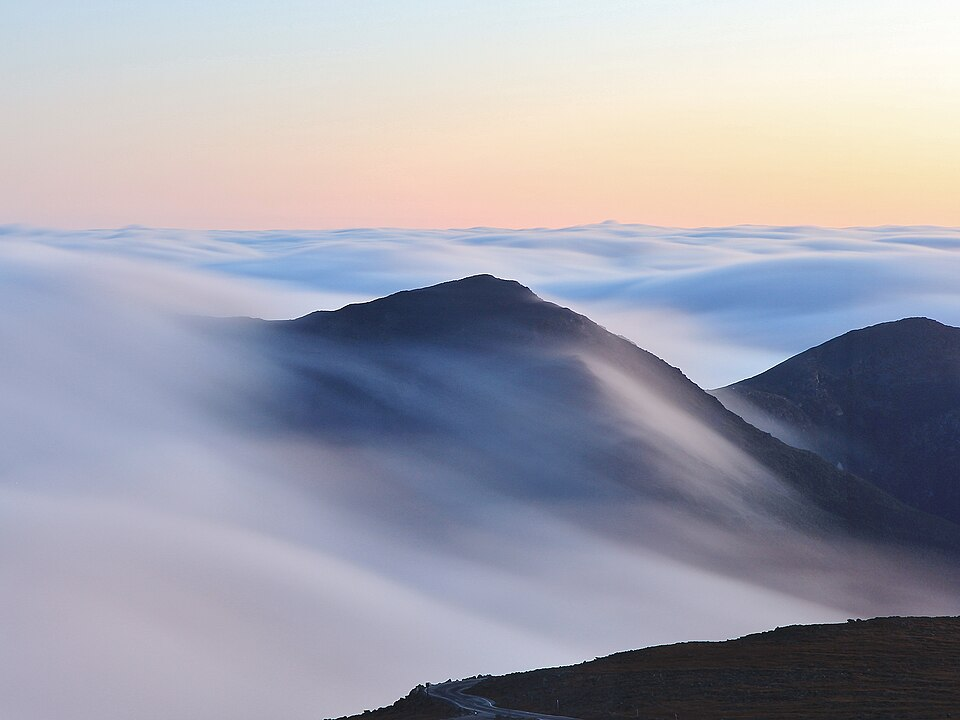
\includegraphics[width=\linewidth]{images/book1/g4-stratus.jpg}

{\small \omterm{def:g4:clouds-rain-snow:cloud-families}{Estratos}: una capa plana, aquí vista desde arriba, desde una
\omterm{def:g1:landscapes-around-us:landform}{montaña}.}
\end{minipage}

\medskip
\begin{minipage}[b]{0.49\linewidth}\centering
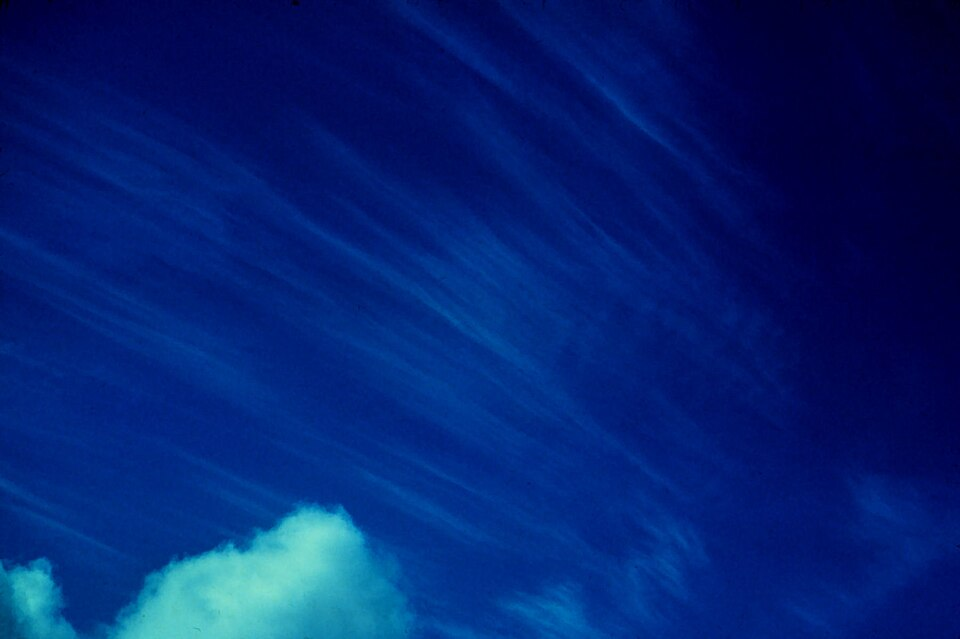
\includegraphics[width=\linewidth]{images/book1/g4-cirrus.jpg}

{\small \omterm{def:g4:clouds-rain-snow:cloud-families}{Cirros}: finos hilos de hielo, muy altos (debajo, un pequeño
\omterm{def:g4:clouds-rain-snow:cloud-families}{cúmulo}).}
\end{minipage}\hfill
\begin{minipage}[b]{0.49\linewidth}\centering
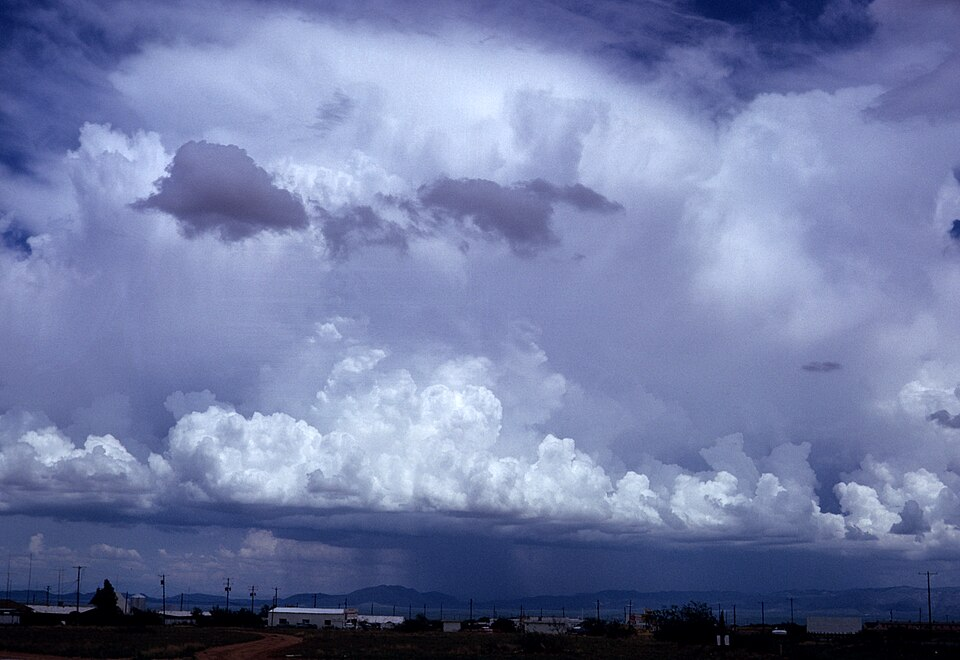
\includegraphics[width=\linewidth]{images/book1/g4-cumulonimbus.jpg}

{\small Un \omterm{def:g4:clouds-rain-snow:cloud-families}{cumulonimbo}: una torre de \omterm{def:g4:clouds-rain-snow:cloud}{nubes}; de su base oscura cae \omterm{def:g4:clouds-rain-snow:precipitation}{lluvia}.}
\end{minipage}

\smallskip
{\small Fotografías: NOAA Photo Library (dominio público): S. Corfidi
(\omterm{def:g4:clouds-rain-snow:cloud-families}{cúmulos}), R. F. Kresge (\omterm{def:g4:clouds-rain-snow:cloud-families}{cirros}), colección B. Hooke (\omterm{def:g4:clouds-rain-snow:cloud-families}{cumulonimbo}).}
% ledger: noaa:photos-g4
\label{fig:g4:clouds-rain-snow:photos}
\end{omfigure}

¿A qué altura flotan las \omterm{def:g4:clouds-rain-snow:cloud}{nubes}? Depende de la familia. Las \omterm{def:g4:clouds-rain-snow:cloud}{nubes} bajas,
como los \omterm{def:g4:clouds-rain-snow:cloud-families}{estratos} y la base de los \omterm{def:g4:clouds-rain-snow:cloud-families}{cúmulos}, flotan desde justo encima del
suelo hasta unos 2 kilómetros. Los \omterm{def:g4:clouds-rain-snow:cloud-families}{cirros} flotan muy alto, entre unos 5 y
13 kilómetros fuera de los trópicos y de las regiones polares --- a menudo
más alto que la \omterm{def:g1:landscapes-around-us:landform}{montaña} más alta de la Tierra.
Un \omterm{def:g4:clouds-rain-snow:cloud-families}{cumulonimbo} se extiende desde una base baja hasta lo más alto de los
niveles de las \omterm{def:g4:clouds-rain-snow:cloud}{nubes}.
% ledger: wmo:cloud-levels, wmo:cumulonimbus

\begin{omfigure}
\begin{tikzpicture}[x=1cm, y=0.5cm, font=\small]
  % height scale
  \draw[black!60] (0,0) -- (0,14);
  \foreach \h in {0,2,...,14} {
    \draw[black!60] (-0.1,\h) -- (0,\h);
    \node[anchor=east, font=\scriptsize] at (-0.12,\h) {\h\,km};
  }
  \node[anchor=south, font=\scriptsize, align=center] at (0,14.2) {altura};
  % ground and a mountain for comparison
  \fill[green!35!black!50] (0.2,0) -- (11.4,0) -- (11.4,-0.4) -- (0.2,-0.4) -- cycle;
  \fill[black!35] (8.6,0) -- (9.9,8.8) -- (10.2,8.4) -- (11.2,0) -- cycle;
  \fill[white, draw=black!45, line width=0.3pt] (9.65,7.2) -- (9.9,8.8) -- (10.2,8.4) -- (10.4,7.0) -- (10.1,7.4) -- (9.9,7.0) -- cycle;
  \node[font=\scriptsize, align=center] at (9.9,10.2) {la montaña\\más alta};
  % levels
  \fill[blue!6] (0.2,0.15) rectangle (8.3,2);
  \fill[blue!10] (0.2,5) rectangle (8.3,13);
  \node[anchor=west, font=\scriptsize, text=blue!50!black] at (0.3,1.65) {nubes bajas};
  \node[anchor=west, font=\scriptsize, text=blue!50!black] at (0.3,12.6) {nubes altas};
  % stratus: a flat grey layer
  \fill[black!25, rounded corners=2pt] (0.6,0.6) rectangle (2.6,1.3);
  \node[font=\scriptsize] at (1.6,-1.1) {estrato};
  % cumulus
  \pic[scale=0.7, transform shape] at (4.0,0.9) {puffycloud};
  \node[font=\scriptsize] at (4.0,-1.1) {cúmulo};
  % cirrus: wisps
  \foreach \y in {9.4,10.0,10.6} {
    \draw[black!50, line width=0.6pt] (0.8,\y) .. controls (1.4,\y+0.5) and (2.0,\y+0.1) .. (2.6,\y+0.6);
  }
  \node[font=\scriptsize] at (1.7,8.5) {cirros};
  % cumulonimbus: tower with an anvil
  \fill[black!15, draw=black!45, line width=0.4pt]
    (5.4,1.0) .. controls (5.2,4) and (5.6,8) .. (5.9,11.2)
    .. controls (5.0,11.6) and (4.6,12.0) .. (4.8,12.3)
    -- (8.1,12.3) .. controls (8.2,12.0) and (7.8,11.6) .. (7.0,11.2)
    .. controls (7.3,8) and (7.6,4) .. (7.4,1.0) -- cycle;
  \fill[black!45] (5.4,1.0) rectangle (7.4,1.4);
  \foreach \x in {5.7,6.1,6.5,6.9,7.2}
    \draw[omWxRain, line width=0.6pt] (\x,0.95) -- (\x-0.15,0.15);
  \node[font=\scriptsize] at (6.4,-1.1) {cumulonimbo};
\end{tikzpicture}

{\small A qué altura flotan las cuatro familias de \omterm{def:g4:clouds-rain-snow:cloud}{nubes} (alturas en
kilómetros, para regiones que no son ni tropicales ni polares). El \omterm{def:g4:clouds-rain-snow:cloud-families}{estrato}
y la base del \omterm{def:g4:clouds-rain-snow:cloud-families}{cúmulo} están bajos; los \omterm{def:g4:clouds-rain-snow:cloud-families}{cirros} suelen estar más altos que la
\omterm{def:g1:landscapes-around-us:landform}{montaña} más alta. Un \omterm{def:g4:clouds-rain-snow:cloud-families}{cumulonimbo} se extiende desde una base baja hasta lo
más alto de los niveles de las \omterm{def:g4:clouds-rain-snow:cloud}{nubes}. Alturas según el atlas de \omterm{def:g4:clouds-rain-snow:cloud}{nubes} de la
Organización Meteorológica Mundial.}
\label{fig:g4:clouds-rain-snow:heights}
% ledger: wmo:cloud-levels, tht:everest
\end{omfigure}

\begin{method}[Poner nombre a una nube]\label{met:g4:clouds-rain-snow:naming}
Mira el cielo y hazte tres preguntas:
\begin{enumerate}
  \item ¿Es un montón de base plana? Entonces es un \omterm{def:g4:clouds-rain-snow:cloud-families}{cúmulo} --- y si se
        eleva en una enorme torre oscura, un \omterm{def:g4:clouds-rain-snow:cloud-families}{cumulonimbo}.
  \item ¿Es una lámina plana y uniforme que tapa todo el cielo? Entonces es
        un \omterm{def:g4:clouds-rain-snow:cloud-families}{estrato}.
  \item ¿Está hecha de finos hilos blancos, muy altos? Entonces es un \omterm{def:g4:clouds-rain-snow:cloud-families}{cirro}.
\end{enumerate}
\end{method}

\begin{remark}[Las nubes anuncian el tiempo]\label{rem:g4:clouds-rain-snow:tell}
Unos \omterm{def:g4:clouds-rain-snow:cloud-families}{cúmulos} pequeños en un cielo azul anuncian buen \omterm{def:g1:watching-the-weather:weather}{tiempo}. Un \omterm{def:g4:clouds-rain-snow:cloud-families}{estrato}
gris trae un día apagado, a veces con llovizna. Un \omterm{def:g4:clouds-rain-snow:cloud-families}{cumulonimbo} trae un
chubasco corto y fuerte, a menudo con truenos, relámpagos y ráfagas de
viento --- a veces \omterm{def:g4:clouds-rain-snow:precipitation}{granizo}. Los \omterm{def:g4:clouds-rain-snow:cloud-families}{cirros} no traen \omterm{def:g4:clouds-rain-snow:precipitation}{lluvia}, pero cuando se
extienden y se espesan, la \omterm{def:g4:clouds-rain-snow:precipitation}{lluvia} suele llegar un día después.
\end{remark}

\section{Lluvia, nieve y granizo}

Dentro de una \omterm{def:g4:clouds-rain-snow:cloud}{nube}, las gotitas diminutas chocan unas con otras y se unen,
o los cristales de hielo crecen a \omterm{def:g1:landscapes-around-us:water}{costa} de las gotitas. Una gota de \omterm{def:g4:clouds-rain-snow:cloud}{nube}, o
un cristal, que ha crecido lo bastante y pesa lo bastante ya no puede
flotar: cae.

\begin{definition}[Precipitación]\label{def:g4:clouds-rain-snow:precipitation}
La \emph{precipitación}\index{precipitacion@precipitación} es el agua que
cae de una \omterm{def:g4:clouds-rain-snow:cloud}{nube} hasta el suelo: \emph{lluvia}\index{lluvia} (gotas de agua
líquida), \emph{nieve}\index{nieve} (copos hechos de cristales de hielo
pegados entre sí) o \emph{granizo}\index{granizo} (bolas de hielo, llamadas
piedras de granizo, que caen de las \omterm{def:g4:clouds-rain-snow:cloud}{nubes} de tormenta).
\end{definition}

Que llueva o que \omterm{def:g4:clouds-rain-snow:precipitation}{nieve} depende de la temperatura del aire que atraviesa la
\omterm{def:g4:clouds-rain-snow:precipitation}{precipitación}. Los copos de \omterm{def:g4:clouds-rain-snow:precipitation}{nieve} se forman muy arriba, en la \omterm{def:g4:clouds-rain-snow:cloud}{nube} fría. Si
el aire de debajo está por encima de \SI{0}{\celsius} durante el tiempo
suficiente, se funden por el camino y nos llegan como \omterm{def:g4:clouds-rain-snow:precipitation}{lluvia}. Si el aire
está bajo cero hasta el suelo, llegan como \omterm{def:g4:clouds-rain-snow:precipitation}{nieve}.

\begin{omfigure}

\includegraphics[width=0.55\linewidth]{images/book1/ai/g4-snowflakes.jpg}

{\small Unos niños atrapan copos de \omterm{def:g4:clouds-rain-snow:precipitation}{nieve} en un guante oscuro: cada copo
está hecho de cristales de hielo.}
\end{omfigure}

El \omterm{def:g4:clouds-rain-snow:precipitation}{granizo} solo cae de los \omterm{def:g4:clouds-rain-snow:cloud-families}{cumulonimbos}. Dentro de la torre, unos vientos
fuertes hacia arriba suben y bajan varias veces unas bolitas de hielo; cada
viaje añade una capa nueva de hielo, como las capas de una cebolla, hasta
que la piedra de \omterm{def:g4:clouds-rain-snow:precipitation}{granizo} pesa demasiado para que el viento la sostenga.

\begin{omfigure}
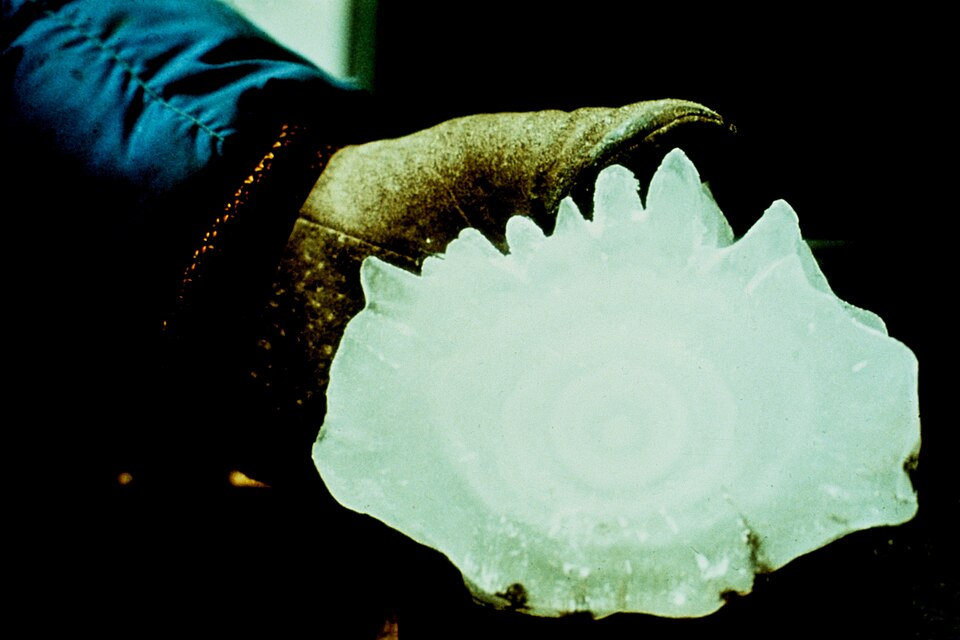
\includegraphics[width=0.5\linewidth]{images/book1/g4-hailstone.jpg}

{\small Una piedra de \omterm{def:g4:clouds-rain-snow:precipitation}{granizo} muy grande en una mano con guante. Los anillos
muestran las capas de hielo que fue acumulando dentro de la \omterm{def:g4:clouds-rain-snow:cloud}{nube} de
tormenta. Fotografía: NOAA Photo Library (dominio público).}
% ledger: noaa:photos-g4
\end{omfigure}

\section{Medir el tiempo}

Para decir cuánto llovió, qué temperatura hizo o de dónde sopló el viento,
las palabras no bastan: necesitamos instrumentos, y números.

\begin{definition}[Pluviómetro]\label{def:g4:clouds-rain-snow:rain-gauge}
Un \emph{pluviómetro}\index{pluviometro@pluviómetro} es un recipiente que
recoge la \omterm{def:g4:clouds-rain-snow:precipitation}{lluvia} que cae sobre su boca. La altura del agua que recoge se
mide en milímetros: ``5 milímetros de \omterm{def:g4:clouds-rain-snow:precipitation}{lluvia}'' quiere decir que la \omterm{def:g4:clouds-rain-snow:precipitation}{lluvia}
habría formado una capa de agua de 5 milímetros de altura sobre un suelo
llano, si nada se hubiera escurrido ni se hubiera filtrado.
\end{definition}

\begin{remark}[Un milímetro de lluvia es mucha agua]\label{rem:g4:clouds-rain-snow:litre}
Un milímetro de \omterm{def:g4:clouds-rain-snow:precipitation}{lluvia} parece muy poco en el \omterm{def:g4:clouds-rain-snow:rain-gauge}{pluviómetro}. Pero sobre un
cuadrado de suelo de un metro por un metro, es un litro de agua: una botella
grande. En un patio de colegio de mil metros cuadrados, una \omterm{def:g4:clouds-rain-snow:precipitation}{lluvia} de
10 milímetros trae diez mil litros: bastan para llenar mil cubos de
10 litros cada uno.
\end{remark}

\begin{omfigure}
\begin{tikzpicture}[font=\small]
  % funnel
  \draw[black!70, line width=0.8pt] (-1.2,6.6) -- (-0.35,5.8) -- (-0.35,5.4);
  \draw[black!70, line width=0.8pt] (1.2,6.6) -- (0.35,5.8) -- (0.35,5.4);
  \draw[black!70, line width=0.8pt] (-1.2,6.6) -- (1.2,6.6);
  % tube
  \fill[blue!25] (-0.45,0) rectangle (0.45,2.4);
  \draw[black!70, line width=0.8pt] (-0.45,5.4) -- (-0.45,0) -- (0.45,0) -- (0.45,5.4);
  \foreach \m in {0,1,...,50} {
    \pgfmathsetmacro{\yy}{\m*0.1}
    \draw[black!60] (0.45,\yy) -- ++(-0.12,0);
  }
  \foreach \m in {0,5,10,...,50} {
    \pgfmathsetmacro{\yy}{\m*0.1}
    \draw[black!80] (0.45,\yy) -- ++(-0.25,0);
    \node[anchor=west, font=\scriptsize] at (0.5,\yy) {\m};
  }
  \node[anchor=west, font=\scriptsize] at (1.0,5.0) {mm};
  % reading line
  \draw[red!70!black, -{Stealth}] (-1.6,2.4) -- (-0.5,2.4);
  \node[anchor=east, align=right, font=\scriptsize] at (-1.65,2.4) {lee el\\nivel aquí};
  \node[anchor=west, font=\scriptsize] at (1.9,2.4) {$\leftarrow$ 24\,mm de lluvia};
\end{tikzpicture}

{\small Un \omterm{def:g4:clouds-rain-snow:rain-gauge}{pluviómetro} sencillo: un embudo recoge la \omterm{def:g4:clouds-rain-snow:precipitation}{lluvia} y un tubo
graduado en milímetros la guarda. Lee el nivel del agua con el ojo a la
misma altura. Aquí han caído 24 milímetros desde la última vez que se vació
el \omterm{def:g4:clouds-rain-snow:rain-gauge}{pluviómetro}.}
\label{fig:g4:clouds-rain-snow:gauge}
\end{omfigure}


\begin{definition}[Veleta]\label{def:g4:clouds-rain-snow:wind-vane}
Una \emph{veleta}\index{veleta} es una flecha que gira libremente sobre un
mástil. El viento empuja su cola, así que la flecha siempre señala la
dirección \emph{de la que} viene el viento.
\end{definition}

\begin{definition}[Estación meteorológica]\label{def:g4:clouds-rain-snow:weather-station}
Una \emph{estación meteorológica}\index{estacion meteorologica@estación meteorológica}
es un lugar donde se mide el \omterm{def:g1:watching-the-weather:weather}{tiempo} cada día, siempre de la misma manera,
con instrumentos: un termómetro en una caseta blanca ventilada, un
\omterm{def:g4:clouds-rain-snow:rain-gauge}{pluviómetro} al aire libre y una \omterm{def:g4:clouds-rain-snow:wind-vane}{veleta} sobre un mástil.
\end{definition}

El termómetro se pone a la sombra, en una caseta blanca de paredes con
lamas que dejan pasar el aire pero no el sol ni la \omterm{def:g4:clouds-rain-snow:precipitation}{lluvia}. La Met Office, el
servicio meteorológico del Reino Unido, la coloca a \SI{1.25}{\metre} del
suelo. El \omterm{def:g4:clouds-rain-snow:rain-gauge}{pluviómetro} está al aire libre, lejos de las paredes y de los
árboles que lo resguardarían de la \omterm{def:g4:clouds-rain-snow:precipitation}{lluvia}, con la boca un poco por encima
del suelo. La \omterm{def:g4:clouds-rain-snow:wind-vane}{veleta} está en lo alto de su mástil, por encima de los
obstáculos que desviarían el viento.
% ledger: mo:screen-height, mo:raingauge

\begin{omfigure}
\begin{tikzpicture}[font=\small, x=1cm, y=1cm]
  % grass
  \fill[green!40!black!45] (-0.5,0) rectangle (11,-0.25);
  \foreach \x in {-0.3,0.1,...,10.8} \draw[green!45!black] (\x,0) -- ++(0.06,0.14);
  % screen on legs
  \draw[black!70, line width=1pt] (0.8,0) -- (0.8,1.25) (2.2,0) -- (2.2,1.25);
  \fill[white, draw=black!70] (0.6,1.25) rectangle (2.4,2.4);
  \foreach \y in {1.4,1.55,...,2.25} \draw[black!40] (0.7,\y) -- (2.3,\y-0.08);
  \fill[white, draw=black!70] (0.45,2.4) -- (1.5,2.75) -- (2.55,2.4) -- cycle;
  \draw[black!60, <->] (2.8,0) -- node[right, font=\scriptsize, align=left] {unos\\1.25\,m} (2.8,1.25);
  \node[align=center, font=\scriptsize] at (1.5,3.25) {termómetro en una\\caseta blanca de lamas};
  % rain gauge
  \fill[black!15, draw=black!70] (5.4,0) rectangle (5.9,0.4);
  \draw[black!70] (5.3,0.55) -- (5.4,0.4) (6.0,0.55) -- (5.9,0.4);
  \node[align=center, font=\scriptsize] at (5.65,1.2) {pluviómetro,\\al aire libre};
  % tree far away
  \fill[brown!60!black] (7.3,0) rectangle (7.5,1.3);
  \fill[green!50!black!70] (7.4,2.1) circle (0.85);
  % wind vane on a mast
  \draw[black!70, line width=1pt] (9.8,0) -- (9.8,4.2);
  \draw[black!80, line width=1.4pt, -{Latex[length=3mm]}] (10.6,4.4) -- (9.0,4.4);
  \fill[black!80] (10.6,4.4) -- (10.9,4.65) -- (10.9,4.15) -- cycle;
  \node[align=center, font=\scriptsize] at (9.8,5.05) {veleta en un mástil alto};
  \node[anchor=west, font=\scriptsize, align=left] at (10.1,3.4) {señala de dónde\\viene el viento};
\end{tikzpicture}

{\small Una pequeña \omterm{def:g4:clouds-rain-snow:weather-station}{estación meteorológica}. El termómetro está a la sombra,
en una caseta blanca de paredes con lamas, a unos 1.25 metros por encima de
la hierba; el \omterm{def:g4:clouds-rain-snow:rain-gauge}{pluviómetro} está al aire libre, lejos del árbol; la \omterm{def:g4:clouds-rain-snow:wind-vane}{veleta}
está muy por encima de los obstáculos.}
\label{fig:g4:clouds-rain-snow:station}
% ledger: mo:screen-height
\end{omfigure}

\begin{inthefield}[Una estación meteorológica en el patio]
Muchos colegios tienen una pequeña \omterm{def:g4:clouds-rain-snow:weather-station}{estación meteorológica} en un rincón del
patio. Cada mañana a la misma hora, dos alumnos leen el termómetro, leen y
vacían el \omterm{def:g4:clouds-rain-snow:rain-gauge}{pluviómetro} y anotan hacia dónde señala la \omterm{def:g4:clouds-rain-snow:wind-vane}{veleta}. Semana tras
semana, la clase va reuniendo un registro de su propio \omterm{def:g1:watching-the-weather:weather}{tiempo}.
\end{inthefield}

\begin{omfigure}
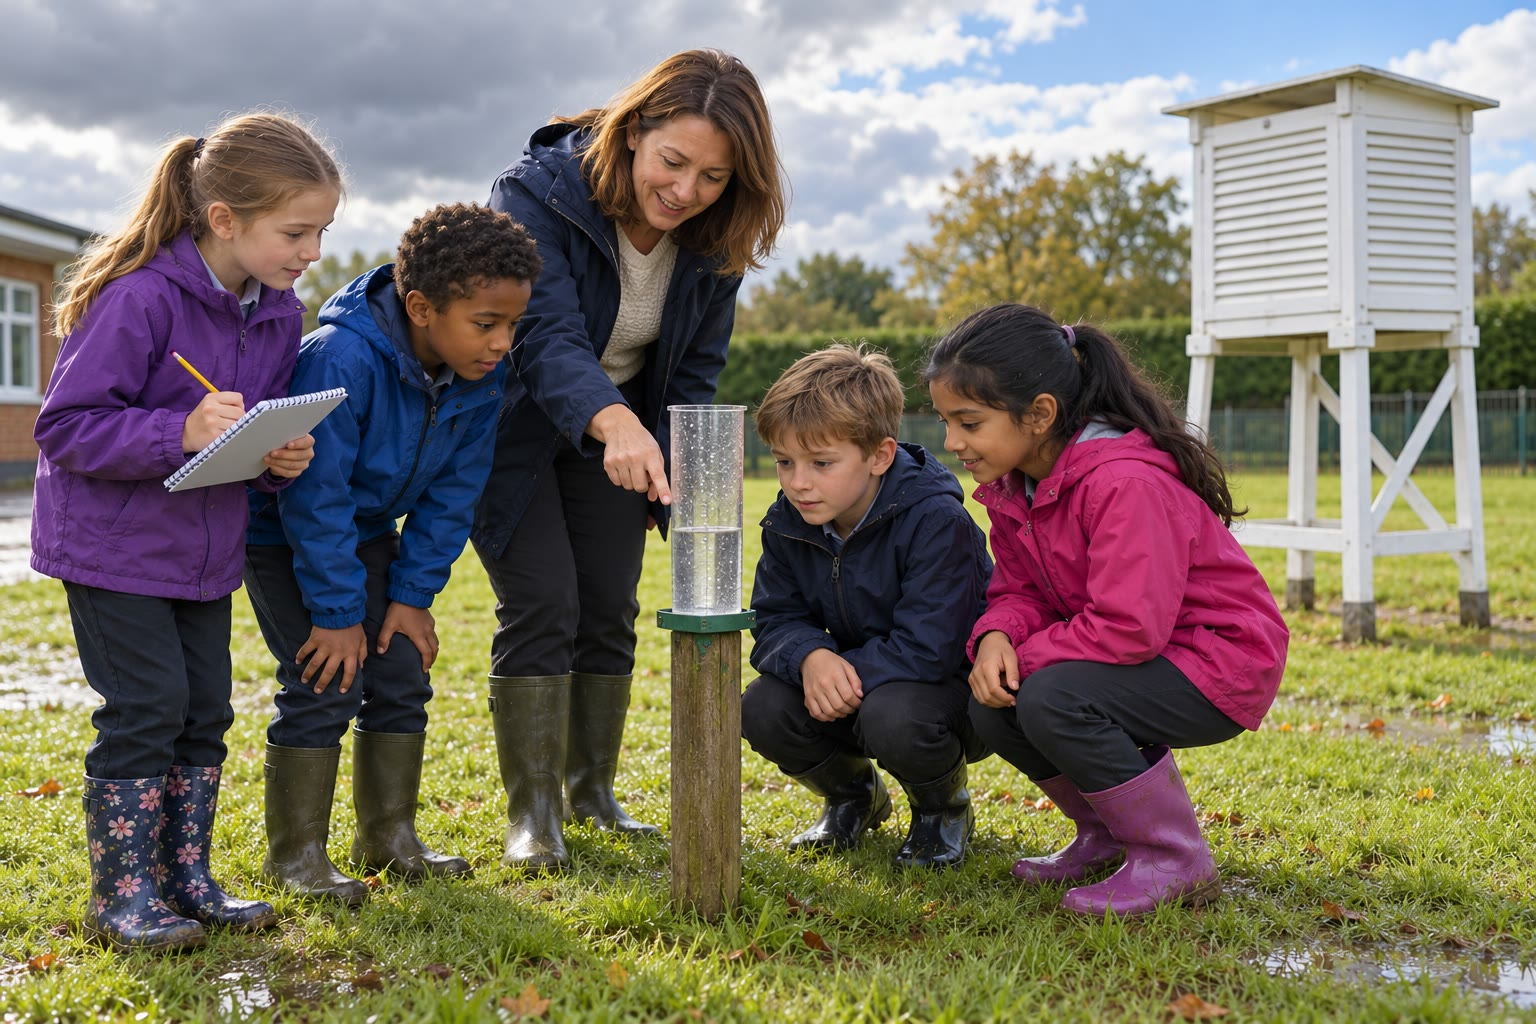
\includegraphics[width=0.55\linewidth]{images/book1/ai/g4-rain-gauge-class.jpg}

{\small Unos alumnos leen el \omterm{def:g4:clouds-rain-snow:rain-gauge}{pluviómetro} en el patio del colegio.}
\end{omfigure}

\begin{method}[Dibujar un diagrama de barras de la lluvia]\label{met:g4:clouds-rain-snow:bar-chart}
Para dibujar la \omterm{def:g4:clouds-rain-snow:precipitation}{lluvia} de una semana:
\begin{enumerate}
  \item traza una línea horizontal y escribe debajo los días, a la misma
        distancia unos de otros;
  \item traza una línea vertical a la izquierda y gradúala en milímetros,
        con pasos iguales (por ejemplo, de 2 en 2 milímetros);
  \item encima de cada día, dibuja una barra tan alta como la \omterm{def:g4:clouds-rain-snow:precipitation}{lluvia} de ese
        día; un día sin \omterm{def:g4:clouds-rain-snow:precipitation}{lluvia} no lleva barra;
  \item ponle un título al diagrama y escribe la unidad, mm, en la línea
        vertical.
\end{enumerate}
\end{method}

\begin{example}[Una semana de lluvia en el colegio]\label{ex:g4:clouds-rain-snow:week}
La clase leyó el \omterm{def:g4:clouds-rain-snow:rain-gauge}{pluviómetro} cada mañana durante una semana y obtuvo: lunes
0, martes 4, miércoles 12, jueves 7, viernes 0, sábado 2 y domingo
5 milímetros. El día más lluvioso fue el miércoles. No llovió ni el lunes
ni el viernes. En toda la semana cayeron
$0 + 4 + 12 + 7 + 0 + 2 + 5 = 30$ milímetros. Solo el miércoles trajo 12 de
los 30 milímetros, es decir, $\frac{12}{30} = \frac{2}{5}$ de la \omterm{def:g4:clouds-rain-snow:precipitation}{lluvia} de
la semana.
\end{example}

\begin{omfigure}
\begin{tikzpicture}
\begin{axis}[ybar, bar width=14pt, width=0.8\linewidth, height=5.4cm,
    ymin=0, ymax=14, ytick={0,2,...,14}, ylabel={lluvia (mm)},
    symbolic x coords={Mon,Tue,Wed,Thu,Fri,Sat,Sun}, xtick=data,
    xticklabels={lun,mar,mié,jue,vie,sáb,dom},
    axis x line*=bottom, axis y line*=left, ymajorgrids, grid style={gray!25},
    nodes near coords, nodes near coords style={font=\scriptsize},
    every axis label/.append style={font=\small}, tick label style={font=\small},
    title={Lluvia en el colegio durante una semana}, title style={font=\small}]
  \addplot[fill=omWxRain!70, draw=omWxRain!60!black] coordinates
    {(Mon,0) (Tue,4) (Wed,12) (Thu,7) (Fri,0) (Sat,2) (Sun,5)};
\end{axis}
\end{tikzpicture}

{\small La semana del \cref{ex:g4:clouds-rain-snow:week} en un diagrama de
barras.}
\label{fig:g4:clouds-rain-snow:bars}
\end{omfigure}

\section{Ejercicios}

\begin{exercise}[$\star$]\label{exo:g4:clouds-rain-snow:1}
¿De qué está hecha una \omterm{def:g4:clouds-rain-snow:cloud}{nube}? ¿Qué es la \omterm{def:g4:clouds-rain-snow:cloud}{niebla}?
\end{exercise}

\begin{exercise}[$\star$]\label{exo:g4:clouds-rain-snow:2}
Di el nombre de la \omterm{def:g4:clouds-rain-snow:cloud}{nube}: (a) una lámina gris y plana que tapa todo el
cielo; (b) finos hilos blancos muy altos en un cielo azul; (c) montones
blancos de base plana, como de algodón; (d) una enorme torre oscura de cima
plana, que trae truenos.
\end{exercise}

\begin{exercise}[$\star$]\label{exo:g4:clouds-rain-snow:3}
¿\omterm{def:g4:clouds-rain-snow:precipitation}{Lluvia}, \omterm{def:g4:clouds-rain-snow:precipitation}{nieve} o \omterm{def:g4:clouds-rain-snow:precipitation}{granizo}? (a) bolas de hielo que caen de una \omterm{def:g4:clouds-rain-snow:cloud}{nube} de
tormenta; (b) gotas de agua líquida; (c) copos hechos de cristales de hielo.
\end{exercise}

\begin{exercise}[$\star$]\label{exo:g4:clouds-rain-snow:4}
¿Qué instrumento mide: (a) la \omterm{def:g4:clouds-rain-snow:precipitation}{lluvia}; (b) la temperatura; (c) de dónde
viene el viento?
\end{exercise}

\begin{exercise}[$\star$]\label{exo:g4:clouds-rain-snow:5}
En el \omterm{def:g4:clouds-rain-snow:rain-gauge}{pluviómetro} dibujado en la página~\pageref{fig:g4:clouds-rain-snow:gauge},
el agua llega ahora a la marca 17. ¿Cuántos milímetros de \omterm{def:g4:clouds-rain-snow:precipitation}{lluvia} han caído?
¿Cuántos milímetros más harían falta para llegar a 20?
\end{exercise}

\begin{exercise}[$\star$]\label{exo:g4:clouds-rain-snow:6}
Mira el diagrama de barras de la página~\pageref{fig:g4:clouds-rain-snow:bars}.
¿Qué día fue el más lluvioso? ¿Qué días no llovió? ¿Qué día cayeron
7 milímetros?
\end{exercise}

\begin{exercise}[$\star\star$]\label{exo:g4:clouds-rain-snow:7}
La mañana de un día de \omterm{def:g4:clouds-rain-snow:precipitation}{nieve}, los copos llegan al suelo en el pueblo de
\omterm{def:g1:landscapes-around-us:landform}{montaña}, pero en el \omterm{def:g1:landscapes-around-us:landform}{valle}, más abajo, llueve. Explica la diferencia usando
la temperatura del aire.
\end{exercise}

\begin{exercise}[$\star\star$]\label{exo:g4:clouds-rain-snow:8}
Otra semana, la clase obtiene: lunes 3, martes 0, miércoles 1, jueves 9,
viernes 6, sábado 0 y domingo 1 milímetros. Dibuja el diagrama de barras.
¿Cuántos milímetros cayeron en la semana? ¿Qué fracción de la \omterm{def:g4:clouds-rain-snow:precipitation}{lluvia} de la
semana cayó el jueves?
\end{exercise}

\begin{exercise}[$\star\star$]\label{exo:g4:clouds-rain-snow:9}
¿Por qué tiene que estar el \omterm{def:g4:clouds-rain-snow:rain-gauge}{pluviómetro} al aire libre, lejos de las paredes
y de los árboles? ¿Por qué se pone el termómetro en una caseta blanca a la
sombra, y no a pleno sol?
\end{exercise}

\begin{exercise}[$\star\star$]\label{exo:g4:clouds-rain-snow:10}
La \omterm{def:g4:clouds-rain-snow:wind-vane}{veleta} señala hacia el oeste. ¿De dónde viene el viento? ¿Hacia dónde
va?
\end{exercise}

\begin{exercise}[$\star\star\star$]\label{exo:g4:clouds-rain-snow:11}
Sobre un patio de 500 metros cuadrados caen 8 milímetros de \omterm{def:g4:clouds-rain-snow:precipitation}{lluvia}. Con la
\cref{rem:g4:clouds-rain-snow:litre}, ¿cuántos litros de agua cayeron sobre
el patio? Una regadera contiene 10 litros: ¿cuántas regaderas son?
\end{exercise}
